% Options for packages loaded elsewhere
\PassOptionsToPackage{unicode}{hyperref}
\PassOptionsToPackage{hyphens}{url}
\PassOptionsToPackage{dvipsnames,svgnames,x11names}{xcolor}
%
\documentclass[
  letterpaper,
  DIV=11,
  numbers=noendperiod]{scrartcl}

\usepackage{amsmath,amssymb}
\usepackage{iftex}
\ifPDFTeX
  \usepackage[T1]{fontenc}
  \usepackage[utf8]{inputenc}
  \usepackage{textcomp} % provide euro and other symbols
\else % if luatex or xetex
  \usepackage{unicode-math}
  \defaultfontfeatures{Scale=MatchLowercase}
  \defaultfontfeatures[\rmfamily]{Ligatures=TeX,Scale=1}
\fi
\usepackage{lmodern}
\ifPDFTeX\else  
    % xetex/luatex font selection
\fi
% Use upquote if available, for straight quotes in verbatim environments
\IfFileExists{upquote.sty}{\usepackage{upquote}}{}
\IfFileExists{microtype.sty}{% use microtype if available
  \usepackage[]{microtype}
  \UseMicrotypeSet[protrusion]{basicmath} % disable protrusion for tt fonts
}{}
\makeatletter
\@ifundefined{KOMAClassName}{% if non-KOMA class
  \IfFileExists{parskip.sty}{%
    \usepackage{parskip}
  }{% else
    \setlength{\parindent}{0pt}
    \setlength{\parskip}{6pt plus 2pt minus 1pt}}
}{% if KOMA class
  \KOMAoptions{parskip=half}}
\makeatother
\usepackage{xcolor}
\usepackage[top=20mm,bottom=20mm,left=20mm,right=20mm]{geometry}
\setlength{\emergencystretch}{3em} % prevent overfull lines
\setcounter{secnumdepth}{-\maxdimen} % remove section numbering
% Make \paragraph and \subparagraph free-standing
\makeatletter
\ifx\paragraph\undefined\else
  \let\oldparagraph\paragraph
  \renewcommand{\paragraph}{
    \@ifstar
      \xxxParagraphStar
      \xxxParagraphNoStar
  }
  \newcommand{\xxxParagraphStar}[1]{\oldparagraph*{#1}\mbox{}}
  \newcommand{\xxxParagraphNoStar}[1]{\oldparagraph{#1}\mbox{}}
\fi
\ifx\subparagraph\undefined\else
  \let\oldsubparagraph\subparagraph
  \renewcommand{\subparagraph}{
    \@ifstar
      \xxxSubParagraphStar
      \xxxSubParagraphNoStar
  }
  \newcommand{\xxxSubParagraphStar}[1]{\oldsubparagraph*{#1}\mbox{}}
  \newcommand{\xxxSubParagraphNoStar}[1]{\oldsubparagraph{#1}\mbox{}}
\fi
\makeatother


\providecommand{\tightlist}{%
  \setlength{\itemsep}{0pt}\setlength{\parskip}{0pt}}\usepackage{longtable,booktabs,array}
\usepackage{calc} % for calculating minipage widths
% Correct order of tables after \paragraph or \subparagraph
\usepackage{etoolbox}
\makeatletter
\patchcmd\longtable{\par}{\if@noskipsec\mbox{}\fi\par}{}{}
\makeatother
% Allow footnotes in longtable head/foot
\IfFileExists{footnotehyper.sty}{\usepackage{footnotehyper}}{\usepackage{footnote}}
\makesavenoteenv{longtable}
\usepackage{graphicx}
\makeatletter
\def\maxwidth{\ifdim\Gin@nat@width>\linewidth\linewidth\else\Gin@nat@width\fi}
\def\maxheight{\ifdim\Gin@nat@height>\textheight\textheight\else\Gin@nat@height\fi}
\makeatother
% Scale images if necessary, so that they will not overflow the page
% margins by default, and it is still possible to overwrite the defaults
% using explicit options in \includegraphics[width, height, ...]{}
\setkeys{Gin}{width=\maxwidth,height=\maxheight,keepaspectratio}
% Set default figure placement to htbp
\makeatletter
\def\fps@figure{htbp}
\makeatother
% definitions for citeproc citations
\NewDocumentCommand\citeproctext{}{}
\NewDocumentCommand\citeproc{mm}{%
  \begingroup\def\citeproctext{#2}\cite{#1}\endgroup}
\makeatletter
 % allow citations to break across lines
 \let\@cite@ofmt\@firstofone
 % avoid brackets around text for \cite:
 \def\@biblabel#1{}
 \def\@cite#1#2{{#1\if@tempswa , #2\fi}}
\makeatother
\newlength{\cslhangindent}
\setlength{\cslhangindent}{1.5em}
\newlength{\csllabelwidth}
\setlength{\csllabelwidth}{3em}
\newenvironment{CSLReferences}[2] % #1 hanging-indent, #2 entry-spacing
 {\begin{list}{}{%
  \setlength{\itemindent}{0pt}
  \setlength{\leftmargin}{0pt}
  \setlength{\parsep}{0pt}
  % turn on hanging indent if param 1 is 1
  \ifodd #1
   \setlength{\leftmargin}{\cslhangindent}
   \setlength{\itemindent}{-1\cslhangindent}
  \fi
  % set entry spacing
  \setlength{\itemsep}{#2\baselineskip}}}
 {\end{list}}
\usepackage{calc}
\newcommand{\CSLBlock}[1]{\hfill\break\parbox[t]{\linewidth}{\strut\ignorespaces#1\strut}}
\newcommand{\CSLLeftMargin}[1]{\parbox[t]{\csllabelwidth}{\strut#1\strut}}
\newcommand{\CSLRightInline}[1]{\parbox[t]{\linewidth - \csllabelwidth}{\strut#1\strut}}
\newcommand{\CSLIndent}[1]{\hspace{\cslhangindent}#1}

\usepackage{fvextra}
\usepackage{float}
\DefineVerbatimEnvironment{Highlighting}{Verbatim}{breaklines,commandchars=\\\{\}}
\pagenumbering{gobble}
\KOMAoption{captions}{tableheading}
\makeatletter
\@ifpackageloaded{caption}{}{\usepackage{caption}}
\AtBeginDocument{%
\ifdefined\contentsname
  \renewcommand*\contentsname{Table of contents}
\else
  \newcommand\contentsname{Table of contents}
\fi
\ifdefined\listfigurename
  \renewcommand*\listfigurename{List of Figures}
\else
  \newcommand\listfigurename{List of Figures}
\fi
\ifdefined\listtablename
  \renewcommand*\listtablename{List of Tables}
\else
  \newcommand\listtablename{List of Tables}
\fi
\ifdefined\figurename
  \renewcommand*\figurename{Figure}
\else
  \newcommand\figurename{Figure}
\fi
\ifdefined\tablename
  \renewcommand*\tablename{Table}
\else
  \newcommand\tablename{Table}
\fi
}
\@ifpackageloaded{float}{}{\usepackage{float}}
\floatstyle{ruled}
\@ifundefined{c@chapter}{\newfloat{codelisting}{h}{lop}}{\newfloat{codelisting}{h}{lop}[chapter]}
\floatname{codelisting}{Listing}
\newcommand*\listoflistings{\listof{codelisting}{List of Listings}}
\makeatother
\makeatletter
\makeatother
\makeatletter
\@ifpackageloaded{caption}{}{\usepackage{caption}}
\@ifpackageloaded{subcaption}{}{\usepackage{subcaption}}
\makeatother

\ifLuaTeX
  \usepackage{selnolig}  % disable illegal ligatures
\fi
\usepackage{bookmark}

\IfFileExists{xurl.sty}{\usepackage{xurl}}{} % add URL line breaks if available
\urlstyle{same} % disable monospaced font for URLs
\hypersetup{
  colorlinks=true,
  linkcolor={blue},
  filecolor={Maroon},
  citecolor={Blue},
  urlcolor={Blue},
  pdfcreator={LaTeX via pandoc}}


\author{}
\date{}

\begin{document}


\section{\texorpdfstring{Black sea bass
(\emph{\texttt{Centropristis\ striata}})}{Black sea bass (Centropristis striata)}}\label{black-sea-bass-centropristis-striata}

\subsection{Summary Scores}\label{summary-scores}

\begin{itemize}
\tightlist
\item
  \textbf{Sensitivity:} Low
\item
  \textbf{Exposure:} Moderate - High
\item
  \textbf{Vulnerability:} Low
\end{itemize}

\subsection{Changes from Previous
Assessment(s)}\label{changes-from-previous-assessments}

\begin{longtable}[]{@{}
  >{\raggedright\arraybackslash}p{(\columnwidth - 6\tabcolsep) * \real{0.2603}}
  >{\raggedright\arraybackslash}p{(\columnwidth - 6\tabcolsep) * \real{0.2329}}
  >{\raggedright\arraybackslash}p{(\columnwidth - 6\tabcolsep) * \real{0.2740}}
  >{\raggedright\arraybackslash}p{(\columnwidth - 6\tabcolsep) * \real{0.2329}}@{}}
\caption{Changes to Vulnerability, Exposure, and Sensitivity scores
relative to Previous Assessments. If a citation for the previous
assessment is not provided, it comes from Hare et al.
(2016).}\tabularnewline
\toprule\noalign{}
\begin{minipage}[b]{\linewidth}\raggedright
Metric
\end{minipage} & \begin{minipage}[b]{\linewidth}\raggedright
Previous Assessment(s)
\end{minipage} & \begin{minipage}[b]{\linewidth}\raggedright
Current Assessment
\end{minipage} & \begin{minipage}[b]{\linewidth}\raggedright
Change
\end{minipage} \\
\midrule\noalign{}
\endfirsthead
\toprule\noalign{}
\begin{minipage}[b]{\linewidth}\raggedright
Metric
\end{minipage} & \begin{minipage}[b]{\linewidth}\raggedright
Previous Assessment(s)
\end{minipage} & \begin{minipage}[b]{\linewidth}\raggedright
Current Assessment
\end{minipage} & \begin{minipage}[b]{\linewidth}\raggedright
Change
\end{minipage} \\
\midrule\noalign{}
\endhead
\bottomrule\noalign{}
\endlastfoot
\emph{Sensitivity} & Moderate & Low & Decrease \\
\emph{Exposure} & Very High & Moderate - High & Decrease \\
\emph{Vulnerability} & High & Low & Decrease \\
\emph{Directional Effect} & Positive & Positive & None \\
\end{longtable}

\newpage{}

\subsection{Stocks}\label{stocks}

\begin{figure}[H]

\centering{

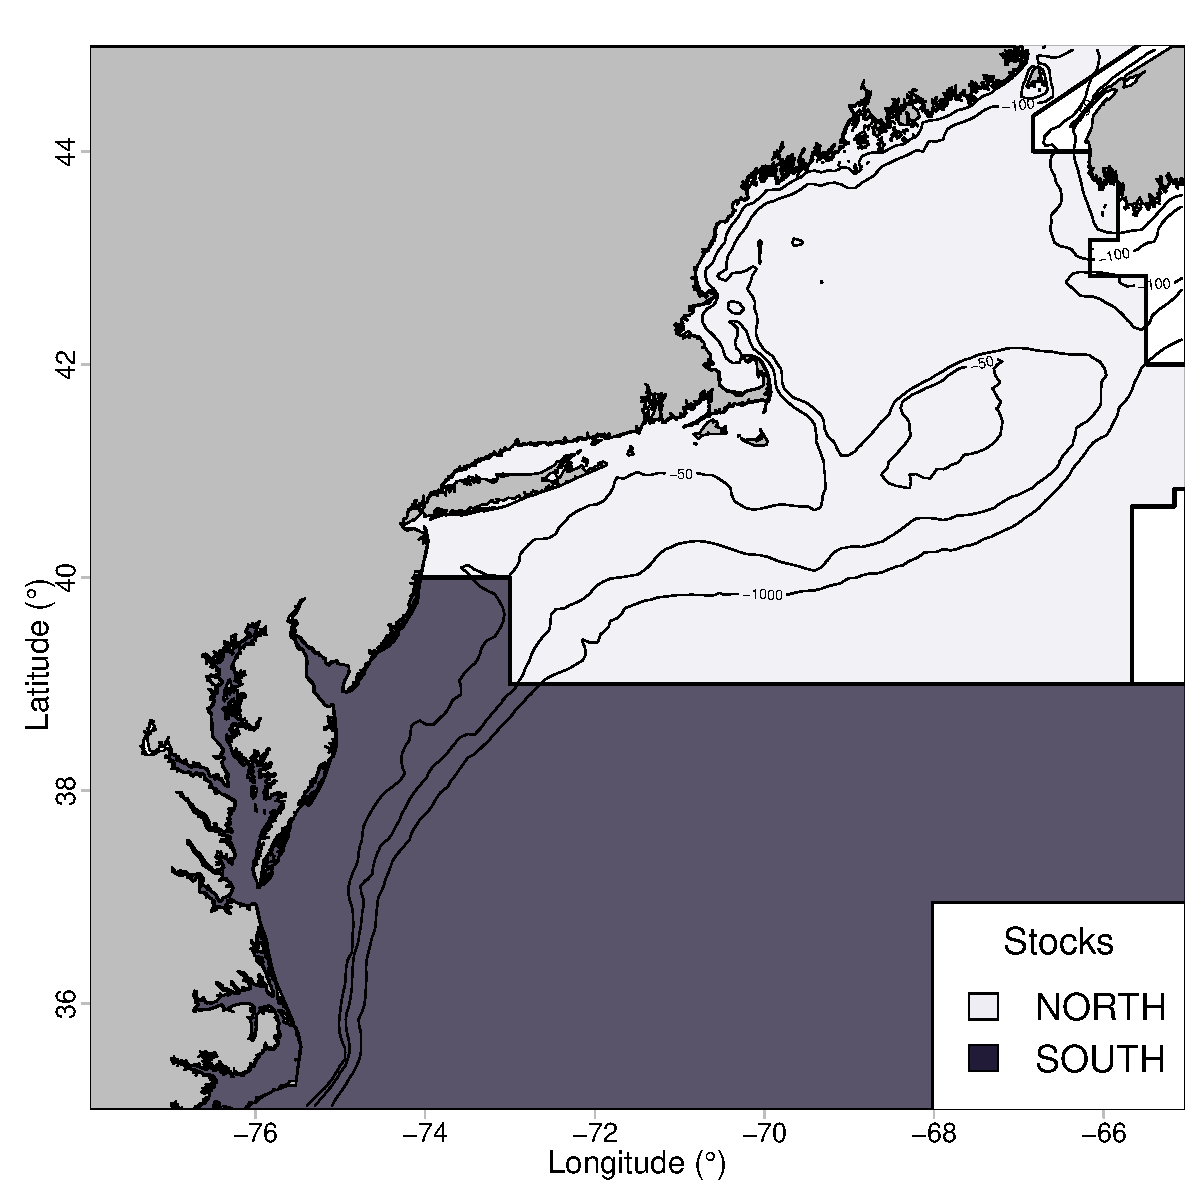
\includegraphics[width=0.85\textwidth,height=\textheight]{../figures/Black sea bass/stock_map_Blackseabass.pdf}

}

\caption{\label{fig-stocks-bsb}Black sea bass Stocks along the Northeast
Shelf}

\end{figure}%

\subsection{Score Descriptions:}\label{score-descriptions}

\subsubsection{Sensitivity:}\label{sensitivity}

\begin{figure}[H]

\centering{

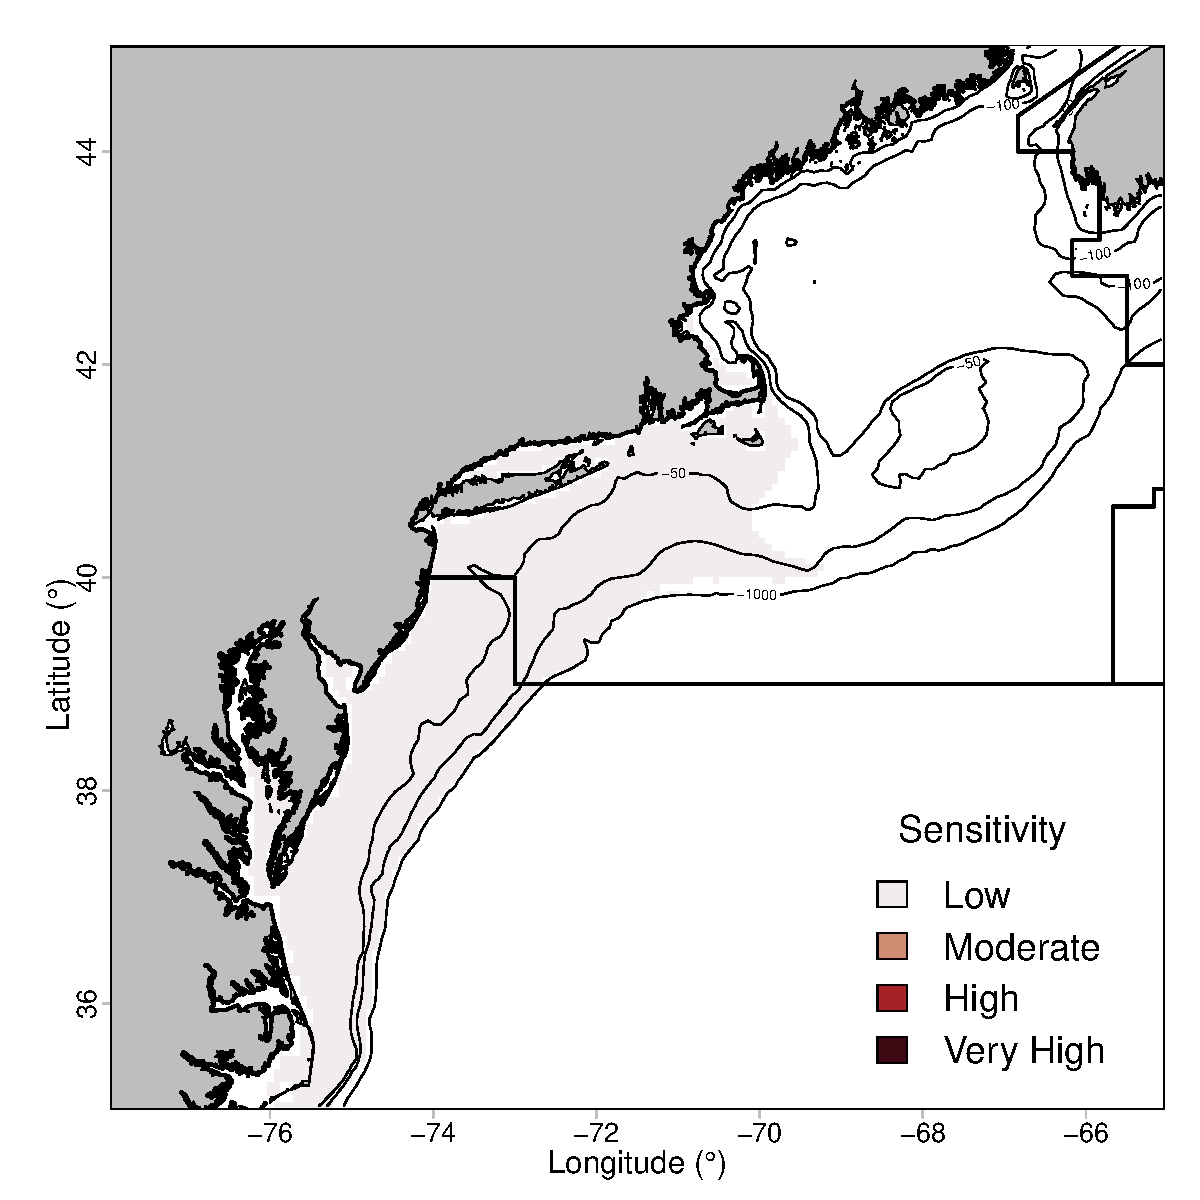
\includegraphics[width=0.85\textwidth,height=\textheight]{../figures/Black sea bass/Blackseabass_sensitivity_2.0.pdf}

}

\caption{\label{fig-sens-bsb}Black sea bass Sensitivity on the Northeast
Shelf}

\end{figure}%

Black Sea Bass received a \textbf{Low} sensitivity score
(\textbf{?@fig-sum-tab-bsb}). Certainty was 64\%. The only score greater
than 2.5 was Complexity in Reproductive Strategy (2.7). This is likely
because black sea bass as protogynous hermaphrodites (they transition
from female to male as they age). Black Sea Bass also spawn in
aggregations that consist of a single dominant male and many females
(Tabandera et al. 2024).

In the 2016 Climate Vulnerability Assessment, Black Sea Bass received a
Moderate sensitivity score. This was driven by Complexity in
Reproductive Strategy (which received the same score in both
assessments) and Early Life History Requirements (Hare et al. 2016).
Juvenile Habitat Requirements was likely important because Black Sea
Bass rely on seagrasses and shellfish beds as nursery habitats (Guyant
et al. 2022). This attribute received a score of 2.4 in our assessment.

\subsubsection{Exposure:}\label{exposure}

\begin{figure}[H]

\centering{

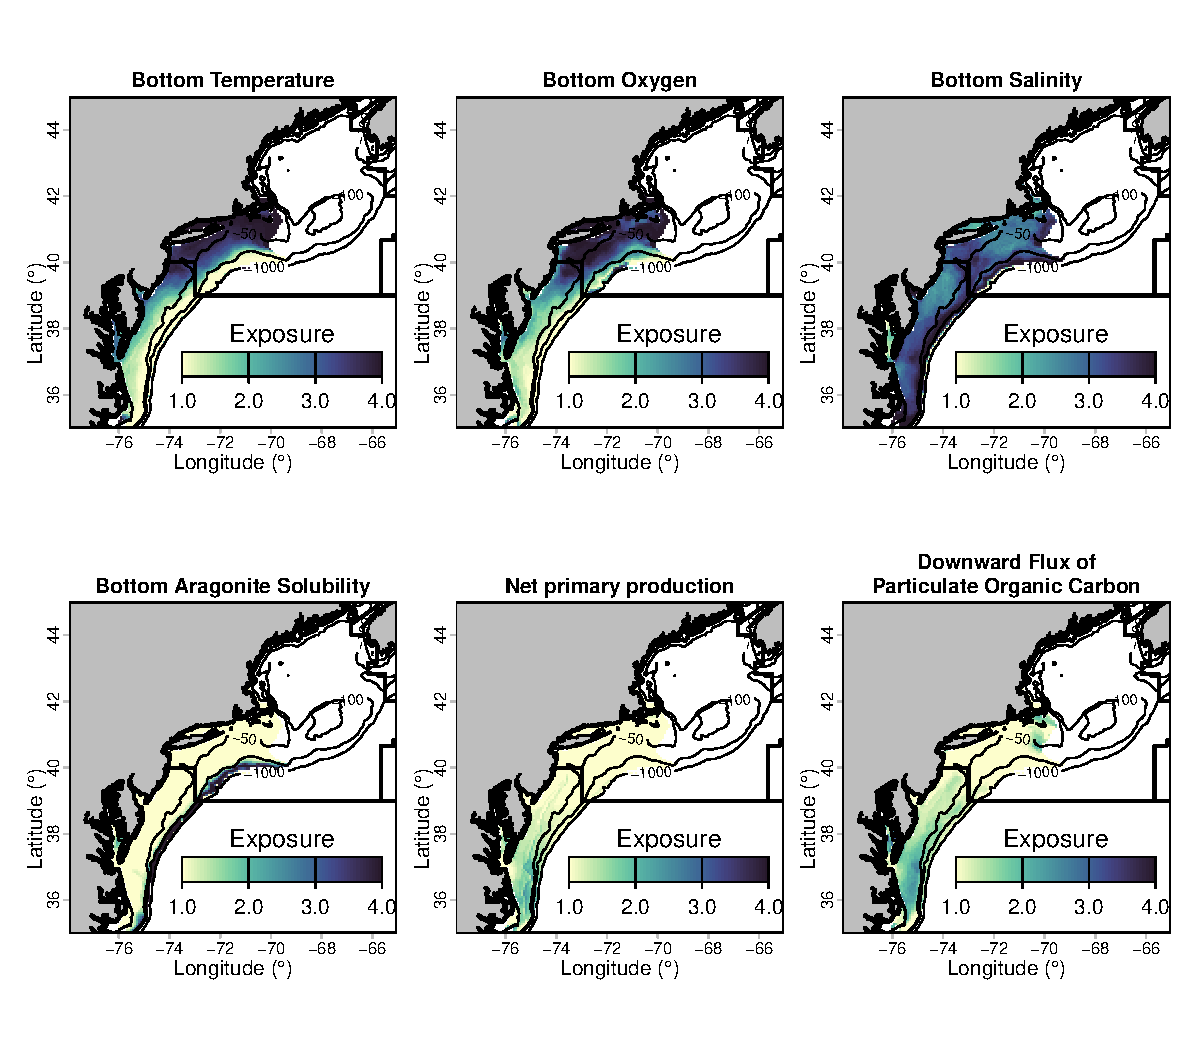
\includegraphics[width=0.85\textwidth,height=\textheight]{../figures/Black sea bass/variable_exposure_maps_r20250925_i202501_r20250715_20142023.pdf}

}

\caption{\label{fig-fact-exp-bsb}Maps of each Exposure Factor for Black
sea bass. Exposure was calculated between 2014-2023 and 2025-2035}

\end{figure}%

Mean Exposure for Black Sea Bass was \textbf{Moderate} throughout its
range (2.02 +/- 0.99) (\textbf{?@fig-sum-tab-bsb}). In the northern half
of its range, exposure was High (2.61 +/- 0.83) whereas it remained
Moderate in the southern half of its range (1.5 +/- 0.80)
(\textbf{?@fig-sum-tab-bsb}). Exposure was greatest south of Cape Cod
and remained high south in Southern New England
(Figure~\ref{fig-exp-bsb}). This was driven by high exposure to changes
in bottom temperature and oxygen (Figure~\ref{fig-fact-exp-bsb}).
Exposure was Low south of New Jersey, with the exception of the
continental shelf, driven by high exposure to changes in bottom
aragonite solubility along the shelf break (Figure~\ref{fig-exp-bsb},
Figure~\ref{fig-fact-exp-bsb}).

In the previous Assessment, Black Sea Bass received a Very High Exposure
score, driven by high exposure to sea surface temperature, air
temperature, and ocean acidification (Hare et al. 2016).

\begin{figure}[H]

\centering{

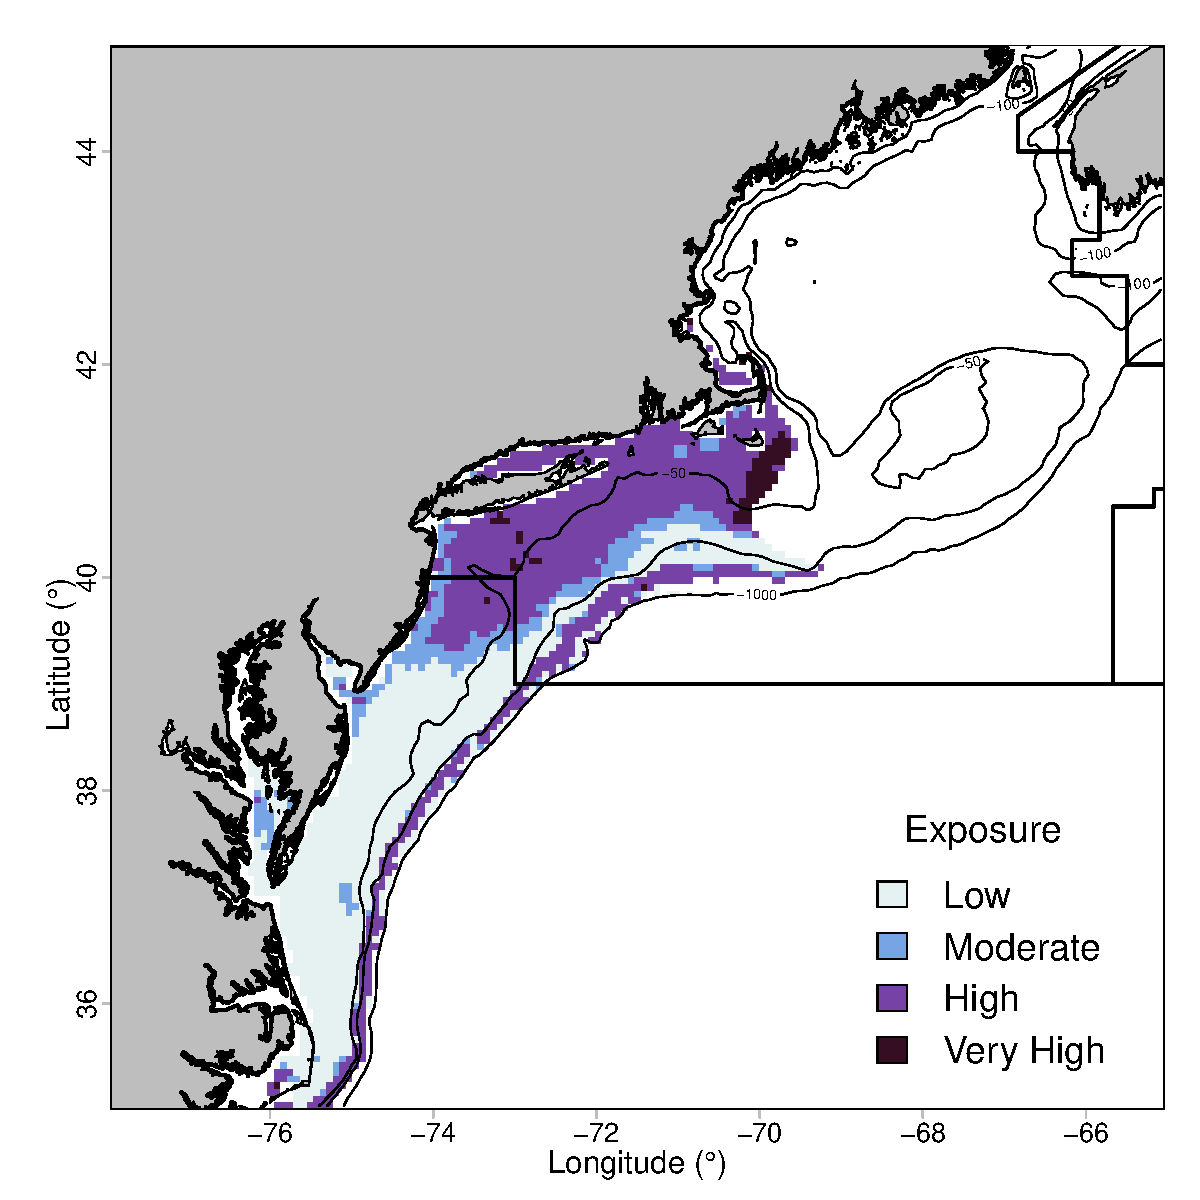
\includegraphics[width=0.85\textwidth,height=\textheight]{../figures/Black sea bass/total_exposure_map_only_all_var_r20250925_i202501_r20250715_20142023.pdf}

}

\caption{\label{fig-exp-bsb}Total Exposure on the Northeast Shelf for
Black sea bass. Total Exposure is calculated by applying the logic rule
from Hare et al. (2016) within grid cells across exposure factors (see
Figure~\ref{fig-fact-exp-bsb})}

\end{figure}%

\subsubsection{Vulnerability:}\label{vulnerability}

\begin{figure}[H]

\centering{

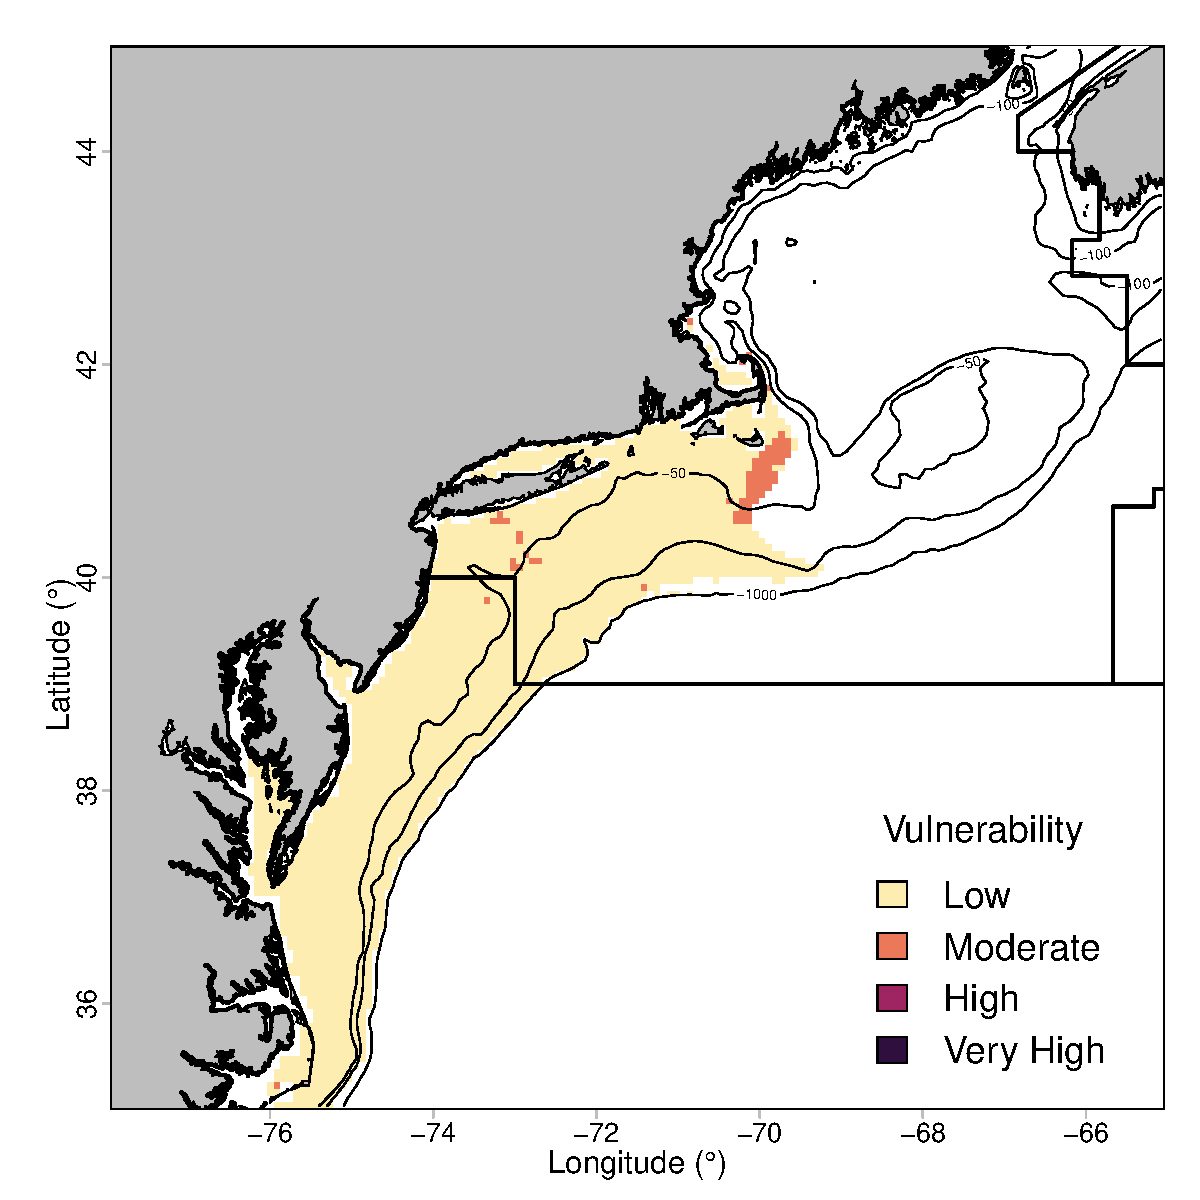
\includegraphics[width=0.85\textwidth,height=\textheight]{../figures/Black sea bass/total_vulnerability_map_only_all_var_r20250925_i202501_r20250715_20142023.pdf}

}

\caption{\label{fig-vuln-bsb}Vulnerability on the Northeast Shelf for
Black sea bass. Vulnerability is the product of sensitivity and exposure
(see Figure~\ref{fig-exp-bsb} and Figure~\ref{fig-sens-bsb})}

\end{figure}%

The mean Vulnerability score for Black Sea Bass was \textbf{Low}
throughout its range and in both the Northern and Southern substocks
(2.02 +/- 0.99) (\textbf{?@fig-sum-tab-bsb}).

Overall vulnerability rank in the previous assessment was High (Hare et
al. 2016).

\subsection{Data Quality Metrics}\label{data-quality-metrics}

\subsubsection{Life History Data
Quality:}\label{life-history-data-quality}

95\% of data quality scores were greater than or equal to 2, indicating
excellent data quality. No data gaps (mean attribute data quality score
\textless{} 2) were identified.

\subsubsection{Model Confidence Score:}\label{model-confidence-score}

The black sea bass ensemble model received a 1.7 (+/- 0.4) model
confidence score, indicating low confidence in the model. Experts stated
that the model described black sea bass distributions well, particularly
in the Mid-Atlantic, but did not represent the recent northern range
expansion. The ensemble model AUC was 0.93, indicating excellent model
performance.

\subsection{Additional Metrics}\label{additional-metrics}

\subsubsection{Distribution Shifts:}\label{distribution-shifts}

\begin{figure}[H]

\centering{

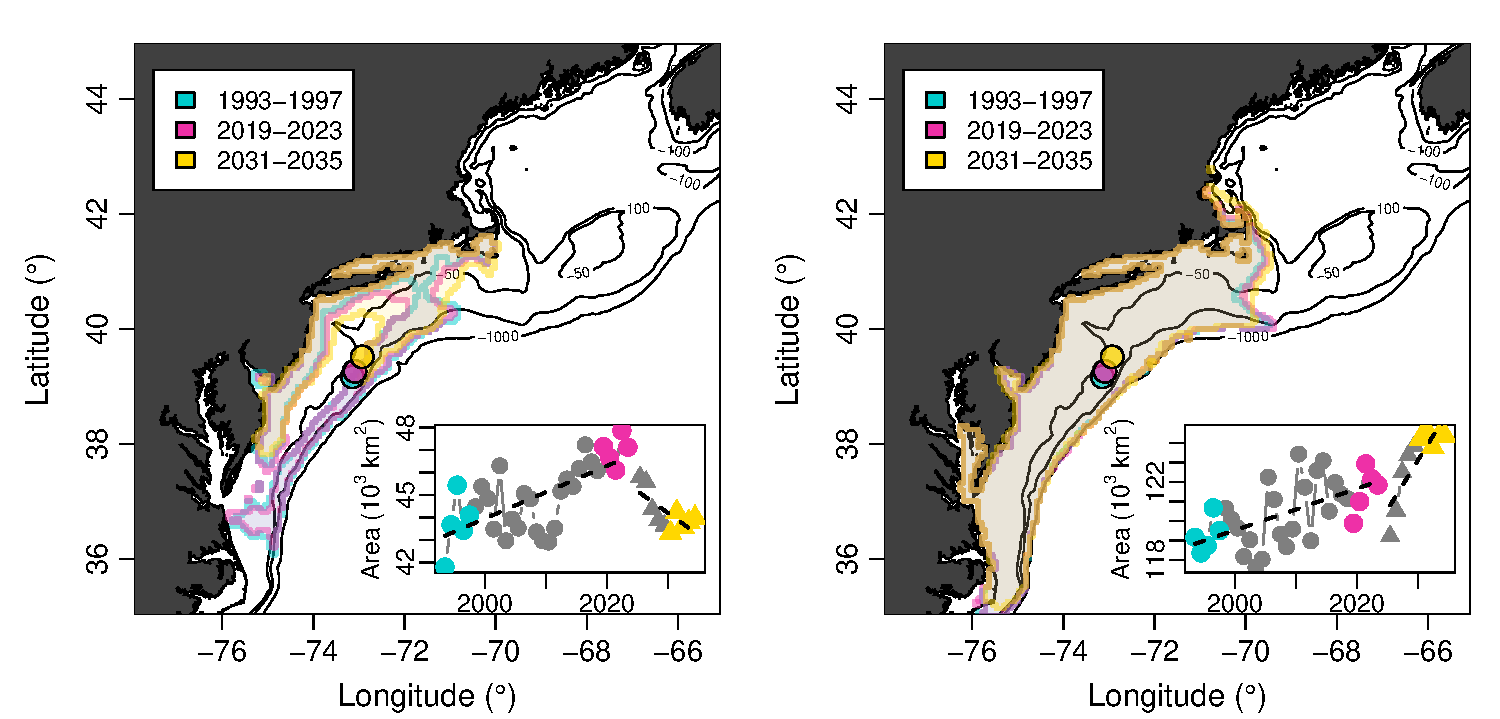
\includegraphics[width=0.85\textwidth,height=\textheight]{../figures/Black sea bass/distribution_shifts_static_r20250715_r20250925_i202501.pdf}

}

\caption{\label{fig-shifts-bsb}Distribution shifts on the Northeast
Shelf for Black sea bass. Polygons illustrate core habitat (left) and
species range (right) for five-year average periods. Points illustrate
weighted centroid, calculated as the average position with species
distribution models as weights. Inset timeseries illustrate the shift in
core and habitat range area over time. Circles represent points from the
MOM6 hindcast; triangles represent points from the MOM6 forecast. Dashed
lines represent significant linear regressions}

\end{figure}%

\emph{Note: For an animated version of this plot, please see the online
version of this document.}

Black sea bass habitat grew significantly between 1993 and 2023. Both
the northern and southern edges of black sea bass distribution shifted
northward. Distributions have also expanded eastward along the coast of
southern New England (Figure~\ref{fig-shifts-bsb}). The weighted
centroid shifted nearly 12 km north-northeast during this time.

There is a predicted loss of core black sea bass habitat along the
continental shelf break. However, total habitat area is predicted to
continue to increase between 2025 and 2035 due to continued northward
expansion into the Gulf of Maine and Cape Cod
(Figure~\ref{fig-shifts-bsb}). The weighted centroid is predicted to
continue to shift a further 31 km north-northeast.

In the previous Assessment, black sea bass received a High
Distributional Vulnerability Rank due to high adult mobility and high
dispersal of eggs and larvae (Hare et al. 2016).

\begin{longtable}[]{@{}
  >{\raggedright\arraybackslash}p{(\columnwidth - 10\tabcolsep) * \real{0.1667}}
  >{\raggedright\arraybackslash}p{(\columnwidth - 10\tabcolsep) * \real{0.1667}}
  >{\raggedright\arraybackslash}p{(\columnwidth - 10\tabcolsep) * \real{0.1667}}
  >{\raggedright\arraybackslash}p{(\columnwidth - 10\tabcolsep) * \real{0.1667}}
  >{\raggedright\arraybackslash}p{(\columnwidth - 10\tabcolsep) * \real{0.1667}}
  >{\raggedright\arraybackslash}p{(\columnwidth - 10\tabcolsep) * \real{0.1667}}@{}}
\caption{Distribution shifts based on five-year average distributions.
Changes are calculated relative to the previous time
period.}\tabularnewline
\toprule\noalign{}
\begin{minipage}[b]{\linewidth}\raggedright
Time Period
\end{minipage} & \begin{minipage}[b]{\linewidth}\raggedright
Weighted Centroid Shift (km \& bearing)
\end{minipage} & \begin{minipage}[b]{\linewidth}\raggedright
Core Habitat Area (change) (km\textsuperscript{2})
\end{minipage} & \begin{minipage}[b]{\linewidth}\raggedright
Habitat Total Area (change) (km\textsuperscript{2})
\end{minipage} & \begin{minipage}[b]{\linewidth}\raggedright
Latitude Range (change) (deg)
\end{minipage} & \begin{minipage}[b]{\linewidth}\raggedright
Change in Longitude Range (deg)
\end{minipage} \\
\midrule\noalign{}
\endfirsthead
\toprule\noalign{}
\begin{minipage}[b]{\linewidth}\raggedright
Time Period
\end{minipage} & \begin{minipage}[b]{\linewidth}\raggedright
Weighted Centroid Shift (km \& bearing)
\end{minipage} & \begin{minipage}[b]{\linewidth}\raggedright
Core Habitat Area (change) (km\textsuperscript{2})
\end{minipage} & \begin{minipage}[b]{\linewidth}\raggedright
Habitat Total Area (change) (km\textsuperscript{2})
\end{minipage} & \begin{minipage}[b]{\linewidth}\raggedright
Latitude Range (change) (deg)
\end{minipage} & \begin{minipage}[b]{\linewidth}\raggedright
Change in Longitude Range (deg)
\end{minipage} \\
\midrule\noalign{}
\endhead
\bottomrule\noalign{}
\endlastfoot
1993-1997 & NA & 44,186 & 119,369 & 5.05 & 5.37 \\
2019-2023 & 11.6 km NNE & 47,354 (+3,168) & 121,620 (+2,251) & 4.99
(-0.06) & 5.53 (+0.16) \\
2031-2035 & 31.2 km NNE & 43,780 (-3,574) & 124,309 (+2,689) & 4.86
(-0.12) & 5.53 (0) \\
\end{longtable}

\subsubsection{Directional Effect:}\label{directional-effect}

Black sea bass are expected to be \textbf{positively} impacted by
climate change. Expert certainty was 100\%. Black sea bass have been
expanding their distributions northward into the Gulf of Maine (McMahan,
Sherwood, and Grabowski 2020), likely due to increasing temperature
supporting recruitment. This is the same result as the 2016 assessment
(Hare et al. 2016).

\subsection{Climate Effects on Abundance and
Distribution}\label{climate-effects-on-abundance-and-distribution}

Black sea bass in the Mid-Atlantic Bight are currently expanding their
distribution northward into the Gulf of Maine (McMahan, Sherwood, and
Grabowski 2020). Black sea bass in their newly-expanded range have a
less diverse diet, lower condition, and a younger age-at-maturity than
their counterparts at the historic northern range of the stock (McMahan,
Sherwood, and Grabowski 2020). A laboratory study on Mid-Atlantic black
sea bass observed a decline in bodily processes that require oxygen
demand above 24°C, suggesting black sea bass will continue to shift
their range poleward with warming conditions (Slesinger et al. 2020).
Tabandera et al. (2024) found that winter bottom temperature was
positively correlated with recruitment deviations in black sea bass.
Black sea bass in the southern Mid-Atlantic Bight also appear to occupy
a smaller portion of their habitat in years with an increase in cold
shelf water on the shelf slope. Northward distributions of black sea
bass are resulting in new species interactions and habitat overlaps. In
Narragansett Bay, black sea bass juveniles now share nursery habitats
with juvenile tautog and cunner, however dietary overlap was
size-dependent and ontogenic diet shifts eventually led to niche
separation (Bell et al. 2015) (Taylor et al. 2023).

\subsection{Life History Synopsis}\label{life-history-synopsis}

Black sea bass are found along the U.S. Atlantic coast from Cape Cod to
the Gulf of America in structured habitats such as reefs, shipwrecks, or
oyster beds (Drohan, Manderson, and Packer 2007). In the Mid-Atlantic
Bight, spawning occurs from April to October, beginning first in the
southern portion of their range and northern latitudes starting later in
the year (Kenneth W. Able and Fahay 1998). Early larval stages last
approximately 72 hrs at 21°C but can last anywhere from 2-6 days
depending on temperature (Berlinsky et al. 2004). Afterwards, larvae
enter a 21-24 day planktonic phase where they can disperse up to 50
miles by currents (Watanabe et al. 2021). Eggs and pelagic larvae are
vulnerable to predation, especially by gelatinous zooplankton (Arai
1988). Larvae settle in nearshore shelf habitats and then migrate to
estuarine nurseries to settle and metamorphose into juveniles (occurs at
13-24mm) (K. W. Able, Fahay, and Shepherd 1995). Larvae are abundant at
temperatures between 13-21°C and leave estuaries for deeper water when
temperatures dip below 14°C (Kendall 1972). Larvae consume microalgae
and zooplankton, including rotifers (Richards 1963). Metamorphosis is
likely the biggest factor influencing settlement (Musick and Mercer
1977). Structural complexity appears to be an essential component of
juvenile black sea bass habitat offshore as well as inshore nurseries
throughout the species range. In offshore areas, recently settled fish
occur in accumulations of shell on sand substrata, complex
microtopographies on exposed clay, on rocky reefs, and on wrecks (K. W.
Able, Fahay, and Shepherd 1995). Primary black sea bass settlement
habitats are probably located along the near shore continental shelf in
accumulations of the shells of bivalves, including Atlantic surfclams
(\emph{Spisula solidissima}) (K. W. Able, Fahay, and Shepherd 1995).
Juvenile growth rates impact winter mortality. Smaller juveniles have
smaller lipid reserves and higher metabolic rates and therefore face
higher predation or starvation risks in the winter (Geissinger et al.
2021). Juveniles, which are diurnal, visual predators, prey on benthic
and epibenthic crustaceans (isopods, amphipods, small crabs, sand
shrimp, copepods, mysids) and small fish. As they mature, their diet
diversifies to include crabs, krill, isopods, shrimp, and small fish
(Kimmel 1973). Adult black sea bass perform seasonal inshore/offshore
migrations between coastal spawning grounds and offshore overwintering
habitats. Migrations are triggered by declining temperatures (around
10-12°C) and begin in the North moving southward (Tabandera et al.
2024). In the Mid-Atlantic Bight, individuals have home ranges as large
as 7km\textsuperscript{2} (Tabandera et al. 2024). Observations suggest
that spawning aggregations consist of a single dominant male and a harem
of females. These spawning aggregations may rely on visual cues rather
than chemical or environmental cues (Tabandera et al. 2024). Black sea
bass are protogynous hermaphrodites, with fish changing sex from female
to male as they increase in age and size (McGovern et al. 2002). Age of
sexual transition varies with latitude with females maturing and
undergoing sexual transition at greater ages in northern latitudes
(O'Brien, Burnett, and Mayo 1993). On average, age at maturity in the
Mid-Atlantic is 2-3 years but can extend up to 5 years (O'Brien,
Burnett, and Mayo 1993). Maximum age for females is 8 years and 12 years
for males (Northeast Fisheries Science Center 2017). The black sea bass
fishery in the Northwest Atlantic is divided into two stock subunits
(north and south) and is managed by the Mid-Atlantic Fishery Management
Council along with the Atlantic States Marine Fisheries Commission. As
of the 2025 Management Track Assessment, the Mid-Atlantic stock is not
overfished or subject to overfishing (Atlantic States Marine Fisheries
Commission (ASMFC) 2025).

\subsection{Supplemental Scores}\label{supplemental-scores}

\subsubsection{Exposure Timeseries}\label{exposure-timeseries}

\begin{figure}[H]

\centering{

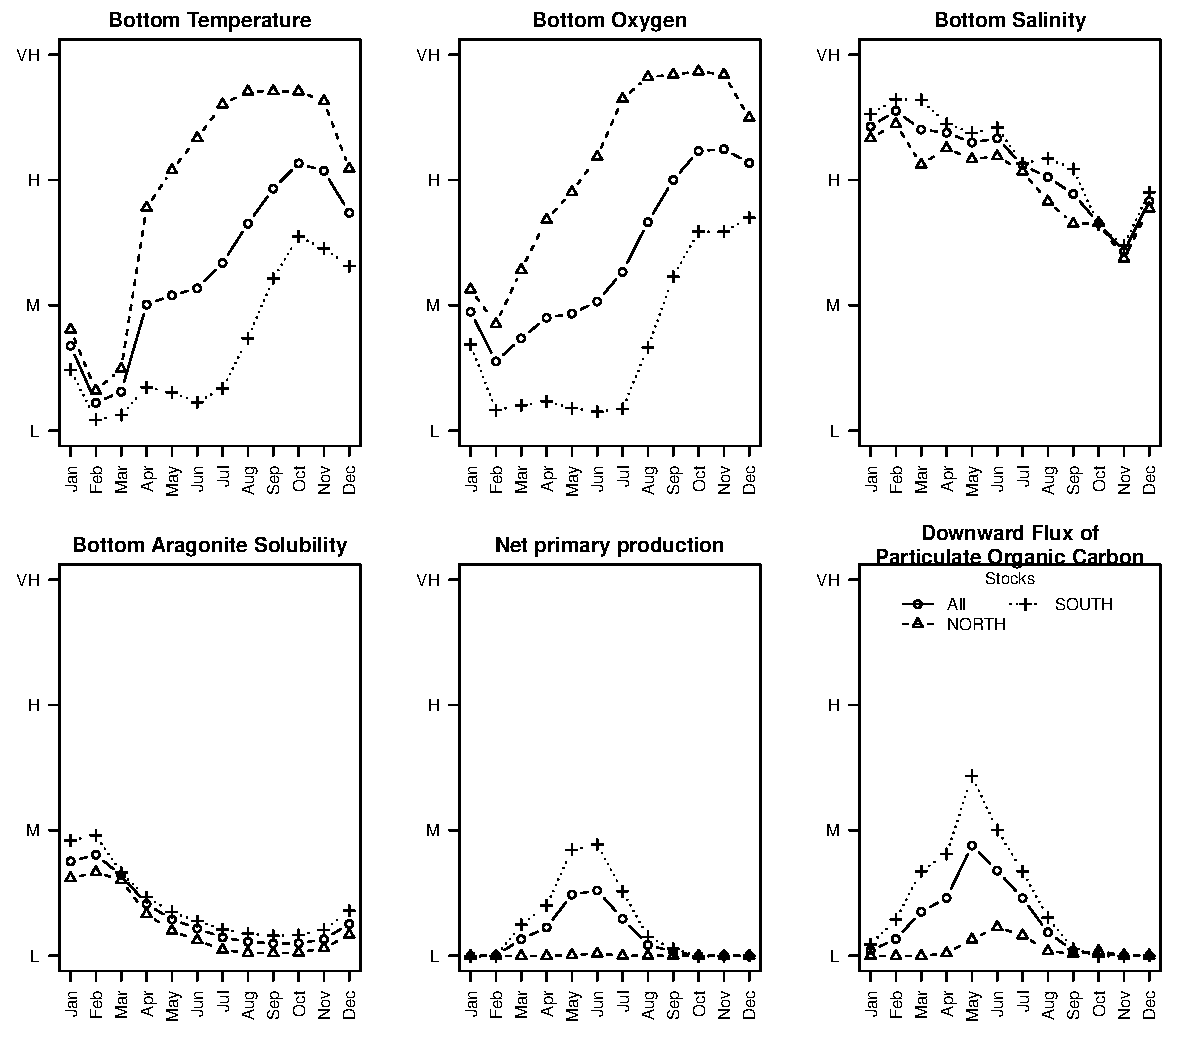
\includegraphics[width=0.85\textwidth,height=\textheight]{../figures/Black sea bass/variable_exposure_timeseries_r20250925_i202501_r20250715_20142023.pdf}

}

\caption{\label{fig-exp-month-tm-bsb}Monthly Timeseries of each Exposure
Factor for Black sea bass. Exposure was calculated between 2014-2023 and
2025-2035}

\end{figure}%

Throughout its range, monthly exposure for black sea bass was Low from
January to July (Figure~\ref{fig-exp-month-bsb}). Exposure increased to
High for October and November. Monthly exposure remained Low throughout
most of the year within the southern half of the range, but was High
from May through December in the northern half
(Figure~\ref{fig-exp-month-bsb}). These patterns were primarily driven
by bottom temperature and oxygen exposure, which was overall higher in
the northern half of the species range
(Figure~\ref{fig-exp-month-tm-bsb}).

\begin{figure}[H]

\centering{

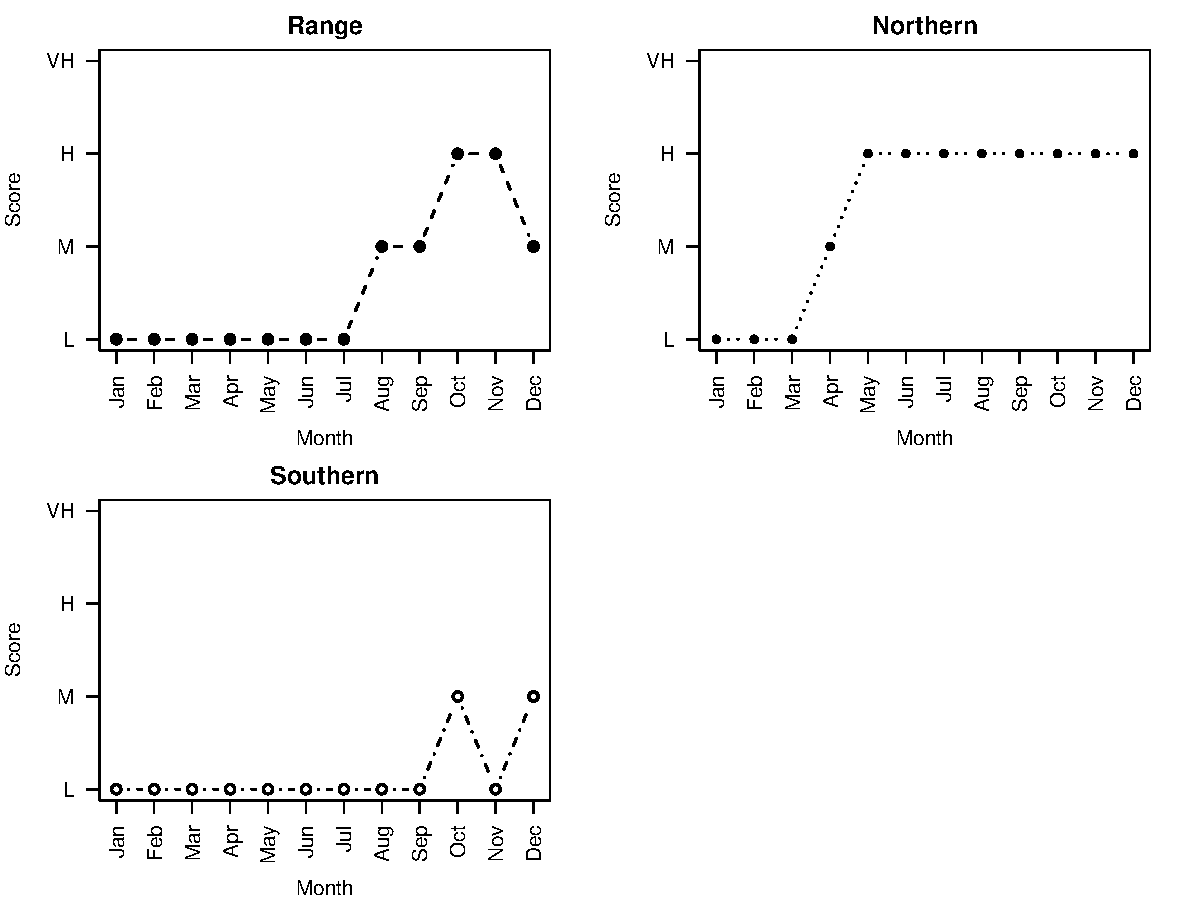
\includegraphics[width=0.85\textwidth,height=\textheight]{../figures/Black sea bass/total_exposure_timeseries_only_all_var_r20250925_i202501_r20250715_20142023.pdf}

}

\caption{\label{fig-exp-month-bsb}Timeseries of Total Exposure for Black
sea bass}

\end{figure}%

\subsubsection{Exposure due to Significant
Factors}\label{exposure-due-to-significant-factors}

\begin{figure}[H]

\centering{

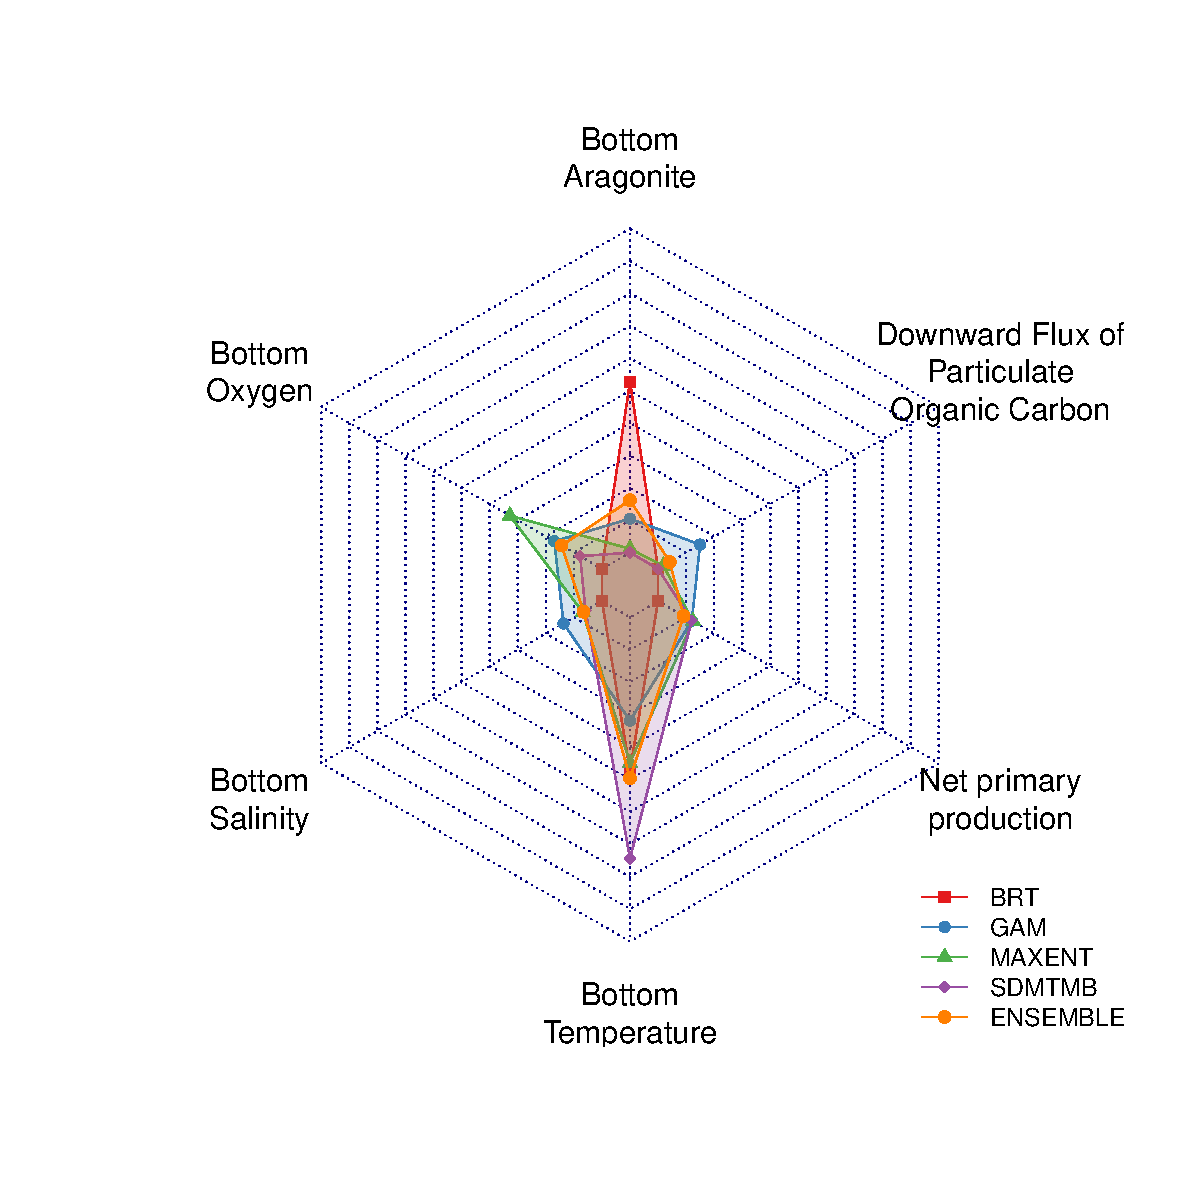
\includegraphics[width=0.85\textwidth,height=\textheight]{../figures/Black sea bass/dynamic_variable_importance_r20250715.pdf}

}

\caption{\label{fig-radar-bsb}Dynamic Factors driving Black sea bass
distributions. The closer the polygon is to the edge of the figure, the
more important the variable is. Each ring represents 10\% variance
explained. Factors must explain at least 10\% of variance in the
ensemble model to be used to calculate total exposure.}

\end{figure}%

Bottom temperature, oxygen, and aragonite solubility were important
dynamic drivers of species distributions (Figure~\ref{fig-radar-bsb}).
Temperature is a known driver of larval development and migration timing
(K. W. Able, Fahay, and Shepherd 1995). Bivalve beds are important
settling habitats, which may drive the importance of aragonite
solubility to species distributions (K. W. Able, Fahay, and Shepherd
1995).

When only these important factors were used to calculate exposure,
scores remained Moderate on average throughout the species range (1.72
+/- 0.92). However, scores decreased from High to Moderate (2.28 +/-
0.92) and Moderate to Low (1.22 +/- 0.58) in the northern and southern
portions of their range, respectively (\textbf{?@fig-sum-imp-bsb}). When
exposure calculations were limited to only important factors, exposure
was greatest south of Long Island and Cape Cod, driven by high
temperature and oxygen exposure (Figure~\ref{fig-exp-imp-bsb}).

\begin{figure}[H]

\centering{

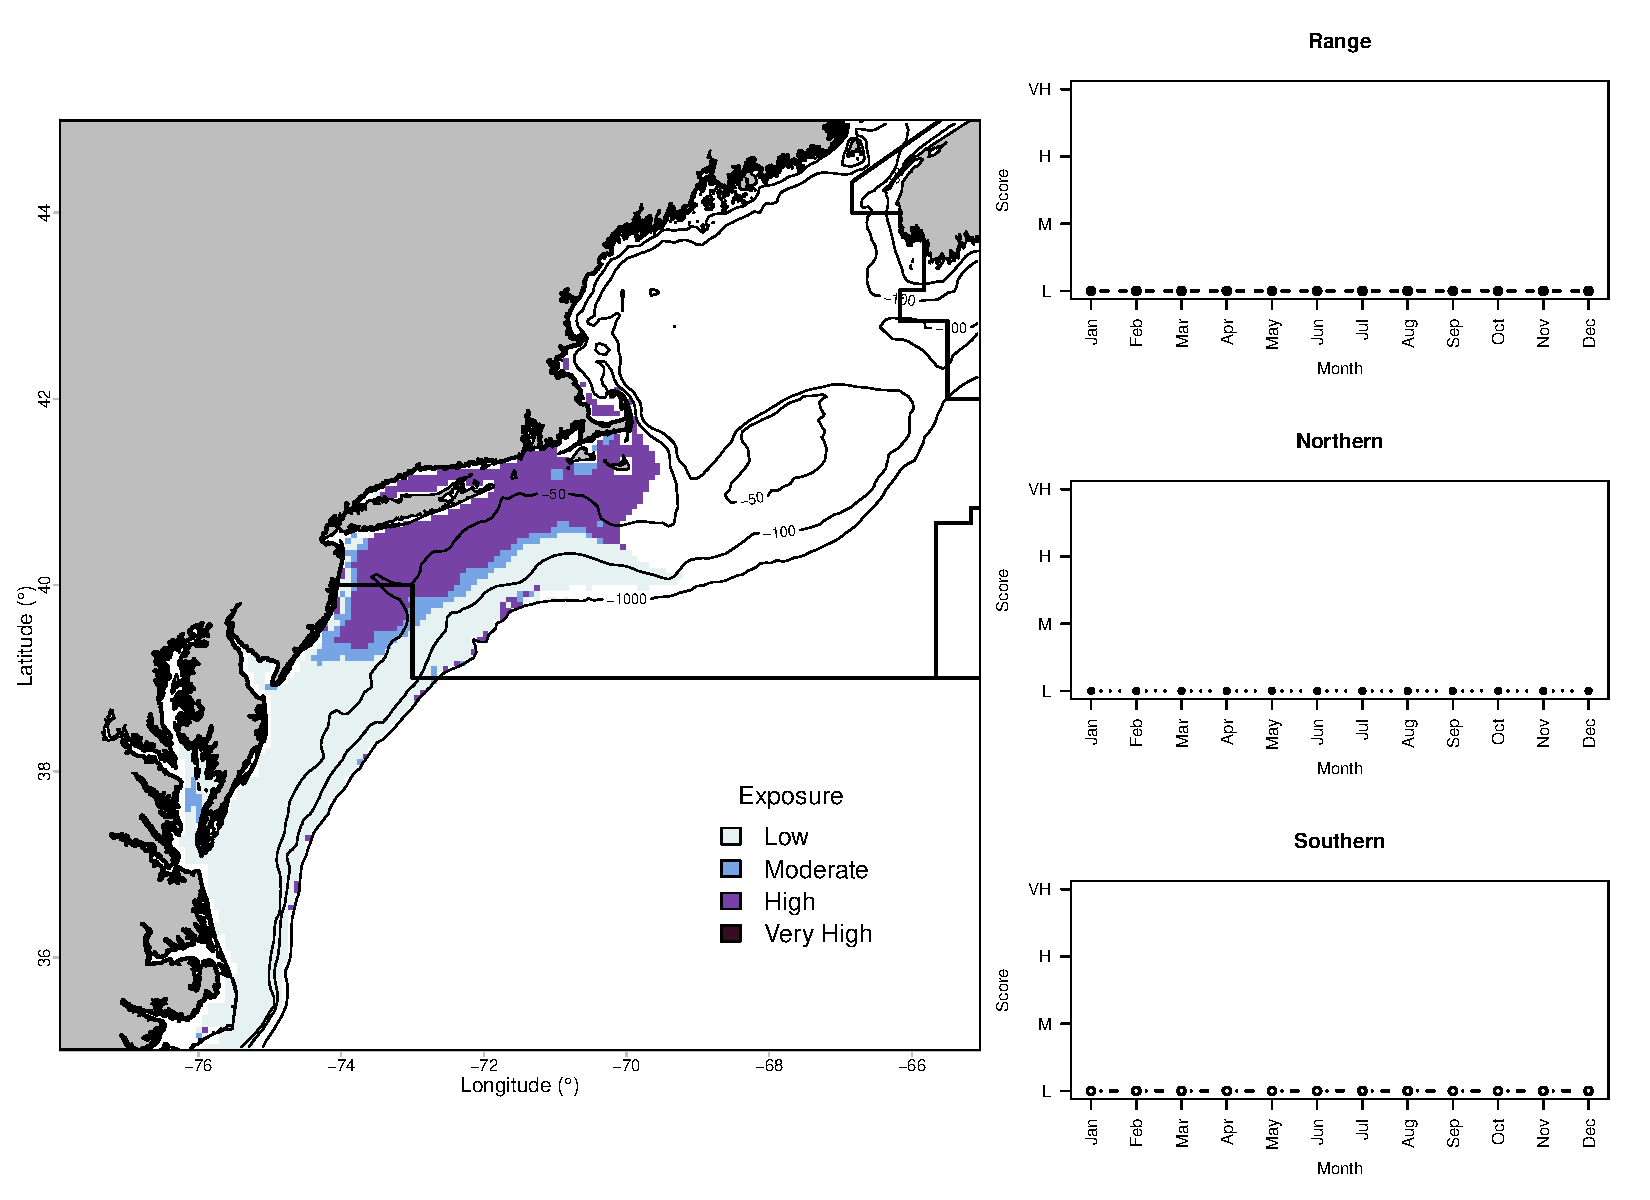
\includegraphics[width=0.85\textwidth,height=\textheight]{../figures/Black sea bass/total_exposure_map_timeseries_imp_var_r20250925_i202501_r20250715_20142023.pdf}

}

\caption{\label{fig-exp-imp-bsb}Total Exposure Map and Timeseries when
Exposure was calculated with only Exposure Factors critical to Black sea
bass distributions}

\end{figure}%

\subsection*{References}\label{references}
\addcontentsline{toc}{subsection}{References}

\phantomsection\label{refs}
\begin{CSLReferences}{1}{0}
\bibitem[\citeproctext]{ref-able1995early}
Able, K. W., M. P. Fahay, and G. R. Shepherd. 1995. {``Early Life
History of Black Sea Bass, {C}entropristis Striata, in the
Mid-{A}tlantic {B}ight and a {N}ew {J}ersey Estuary.''} \emph{Fishery
Bulletin} 93 (3): 429--45.

\bibitem[\citeproctext]{ref-able1998first}
Able, Kenneth W., and Michael P. Fahay. 1998. \emph{The First Year in
the Life of Estuarine Fishes in the Middle Atlantic Bight}. New
Brunswick, NJ: Rutgers University Press.

\bibitem[\citeproctext]{ref-arai1988interactions}
Arai, M. N. 1988. {``Interactions of Fish and Pelagic Coelenterates.''}
\emph{Canadian Journal of Zoology} 66 (9): 1913--27.

\bibitem[\citeproctext]{ref-asmfc2025_bsb}
Atlantic States Marine Fisheries Commission (ASMFC). 2025. {``Black Sea
Bass 2025 Management Track Assessment Report.''} Atlantic States Marine
Fisheries Commission.
\url{https://asmfc.org/wp-content/uploads/2025/08/2025_BSB_MgmtTrackAssmtReport.pdf}.

\bibitem[\citeproctext]{ref-bell2015disentangling}
Bell, R. J., D. E. Richardson, J. A. Hare, P. D. Lynch, and P. S.
Fratantoni. 2015. {``Disentangling the Effects of Climate, Abundance,
and Size on the Distribution of Marine Fish: An Example Based on Four
Stocks from the Northeast US Shelf.''} \emph{ICES Journal of Marine
Science} 72 (5): 1311--22.

\bibitem[\citeproctext]{ref-berlinsky2004effects}
Berlinsky, D. L., J. C. Taylor, R. A. Howell, T. M. Bradley, and T. I.
J. Smith. 2004. {``The Effects of Temperature and Salinity on Early Life
Stages of Black Sea Bass {C}entropristis Striata.''} \emph{Journal of
the World Aquaculture Society} 35: 335--44.
\url{https://doi.org/10.1111/j.1749-7345.2004.tb00097.x}.

\bibitem[\citeproctext]{ref-drohan2007essential}
Drohan, A. F., J. P. Manderson, and D. B. Packer. 2007. {``Essential
Fish Habitat Source Document. {B}lack Sea Bass, {C}entropristis Striata,
Life History and Habitat Characteristics.''} NOAA Technical Memorandum
NMFS-NE 200. \url{https://repository.library.noaa.gov/view/noaa/4038}.

\bibitem[\citeproctext]{ref-geissinger2021food}
Geissinger, E. A., R. S. Gregory, B. J. Laurel, and P. V. Snelgrove.
2021. {``Food and Initial Size Influence Overwinter Survival and
Condition of a Juvenile Marine Fish (Age-0 {A}tlantic Cod).''}
\emph{Canadian Journal of Fisheries and Aquatic Sciences} 78 (4):
472--82.

\bibitem[\citeproctext]{ref-guyant2022northeast}
Guyant, M, M Bachman, J Coakley, G Fay, M Johnson, V Kentner, W
Morrison, and T Rankin. 2022. {``Northeast Regional Habitat
Assessment-Habitat Climate Vulnerability Assessment Crosswalk, Including
Species Narratives, Habitat-Species Matrix, and Final Report.''}
Northeast Regional Habitat Assessment.
\url{https://nrha.shinyapps.io/dataexplorer/\#!/crosswalk}.

\bibitem[\citeproctext]{ref-hare2016vulnerability}
Hare, Jonathan A, Wendy E Morrison, Mark W Nelson, Megan M Stachura,
Eric J Teeters, Roger B Griffis, Michael A Alexander, et al. 2016. {``A
Vulnerability Assessment of Fish and Invertebrates to Climate Change on
the Northeast US Continental Shelf.''} \emph{PloS One} 11 (2): e0146756.

\bibitem[\citeproctext]{ref-kendall1972description}
Kendall, A. W., Jr. 1972. {``Description of Black Sea Bass,
{C}entropristis Striata, ({L}innaeus), Larvae and Their Occurrence North
of {C}ape {L}ookout, {N}orth {C}arolina.''} \emph{Fishery Bulletin
(U.S.)} 70: 1243--59.

\bibitem[\citeproctext]{ref-kimmel1973food}
Kimmel, J. J. 1973. {``Food and Feeding of Fishes from {M}agothy {B}ay,
{V}irginia.''} Master's thesis, Williamsburg, VA: Old Dominion Univ.

\bibitem[\citeproctext]{ref-mcgovern2002temporal}
McGovern, J. C., M. R. Collins, O. Pashuk, and H. S. Meister. 2002.
{``Temporal and Spatial Differences in Life History Parameters of Black
Sea Bass in the Southeastern {U}nited {S}tates.''} \emph{North American
Journal of Fisheries Management} 22 (4): 1151--63.

\bibitem[\citeproctext]{ref-mcmahan2020geographic}
McMahan, M. D., G. D. Sherwood, and J. H. Grabowski. 2020. {``Geographic
Variation in Life-History Traits of Black Sea Bass ({C}entropristis
Striata) During a Rapid Range Expansion.''} \emph{Frontiers in Marine
Science} 7: 567758.

\bibitem[\citeproctext]{ref-musick1977seasonal}
Musick, J. A., and L. P. Mercer. 1977. {``Seasonal Distribution of Black
Sea Bass, {C}entropristis Striata, in the {M}id-{A}tlantic {B}ight with
Comments on the Ecology and Fisheries of the Species.''}
\emph{Transactions of the American Fisheries Society} 106: 12--25.

\bibitem[\citeproctext]{ref-nefsc2017_62saw}
Northeast Fisheries Science Center. 2017. {``62nd {N}ortheast {R}egional
{S}tock {A}ssessment {W}orkshop (62nd {SAW}) {A}ssessment {R}eport.''}
17-03. \url{https://doi.org/10.7289/V5/RD-NEFSC-17-03}.

\bibitem[\citeproctext]{ref-obrien1993maturation}
O'Brien, L., J. Burnett, and R. K. Mayo. 1993. {``Maturation of Nineteen
Species of Finfish Off the Northeast Coast of the {U}nited {S}tates,
1985-1990.''} NOAA Tech. Rep. NMFS 113.

\bibitem[\citeproctext]{ref-richards1963demersal}
Richards, S. W. 1963. {``The Demersal Fish Population of {L}ong {I}sland
{S}ound. {II}. {F}ood of the Juveniles from a Sand-Shell Locality
({S}tation 1).''} \emph{Bulletin of the Bingham Oceanographic
Collection} 18: 32--72.

\bibitem[\citeproctext]{ref-slesinger2020effect}
Slesinger, E., A. Andres, R. Young, B. Seibel, V. Saba, B. Phelan, J.
Rosendale, D. Wieczorek, and G. Saba. 2020. {``The Effect of Ocean
Warming on Black Sea Bass ({C}entropristis Striata) Aerobic Scope and
Hypoxia Tolerance.''} \emph{PLOS ONE} 15 (12): e0244002.
\url{https://doi.org/10.1371/journal.pone.0244002}.

\bibitem[\citeproctext]{ref-tabandera2024black}
Tabandera, R., A. Tyrell, M. McMahan, P. Perez, K. Hankowsky, and S.
Large. 2024. {``Black Sea Bass Ecosystem Considerations and Indicator
Development.''} NOAA Fisheries Northeast Fisheries Science Center.
\url{https://doi.org/10.25923/ez9g-af05}.

\bibitem[\citeproctext]{ref-taylor2023habitat}
Taylor, D. L., C. Pearson, L. Green-Gavrielidis, N. V. Hobbs, C.
Thornber, G. Cicchetti, A. Gerber-Williams, and M. C. McManus. 2023.
{``Habitat and Trophic Niche Overlap Among Juvenile Black Sea Bass,
Tautog, and Cunner: Interspecific Interactions Amid a Species Geographic
Range Expansion.''} \emph{Marine Ecology Progress Series} 720: 133--59.

\bibitem[\citeproctext]{ref-watanabe2021status}
Watanabe, W. O., P. M. Carroll, M. S. Alam, C. F. Dumas, J. E. Gabel, T.
M. Davis, and C. D. Bentley. 2021. {``The Status of Black Sea Bass,
{C}entropristis Striata, as a Commercially Ready Species for {U}.{S}.
Marine Aquaculture.''} \emph{Journal of the World Aquaculture Society}
52 (3): 541--65. \url{https://doi.org/10.1111/jwas.12803}.

\end{CSLReferences}




\end{document}
